\section{Application functionality}
\subsection{Access}
To have access to the application, use the following  command to view the list of all commands with a short description:
\\
\\
\centerline {\code{etherless init}}
%\begin{figure}
%	\centering
%	\includegraphics[width=\textwidth]{res/img/Screenshot_init.jpg}
%	\caption{command list}
%\end{figure}

\subsubsection{Registration}
In order to use the functionality of the Etherless application, the user must be registered into the platform.\\
To do it, you have to use the next command and replace <password>  with a password of your choice.
\\
\centerline{\code{signup <password>}}\\
	\begin{figure}
		\centering
		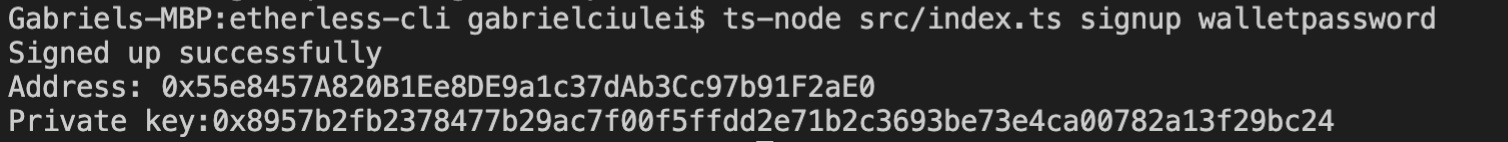
\includegraphics[width=\textwidth]{res/img/Screenshot_signup.png}
		\caption{Signup command}
	\end{figure}\\
\\\\
The system proceeds to register an account and an \textit{Ethereum\glos} wallet  and then returns two values: 
\begin{itemize}
	\item An \textbf{address} associated to the \textit{Ethereum\glos} account;
	\item A \textbf{private-key\glos} associated to the \textit{Ethereum\glos} account.
\end{itemize}
%aggiungere screen del comando 


\subsubsection{Login}
The developer can decide to use an account already existing typing the \textit{private-key\glos} of your own \textit{Ethereum\glos} account already existing and the password chosen.\\\\
\centerline{\code{login <privateKey> <password>}}
\begin{figure}
	\begin{center}
	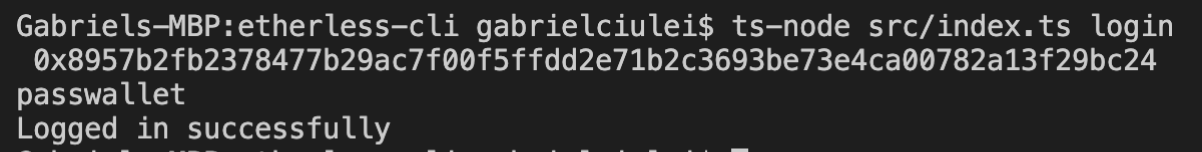
\includegraphics[width=\textwidth]{res/img/Screenshot_login.png}
	\caption{Login command}
	\end{center}
\end{figure}
\\
\\

\subsubsection{Logout}
The user can also disconnect his \textit{Ethereum\glo} account from the \textit{Etherless} application using the command "logout".\\\\
%\centerline{\code{logout}}
\begin{figure}
	\centering
	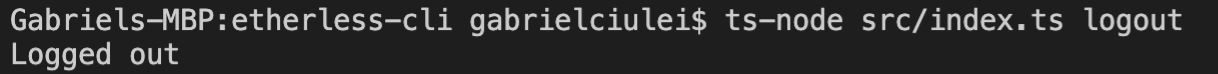
\includegraphics[width=\textwidth]{res/img/Screenshot_logout.png}
	\caption{Logout command}
\end{figure}
\\


\subsection{Commands guide}
\subsubsection{List}
Use the command "list" to view all the available functions deployed\glo to \textit{etherless-server}.\\\\
%\centerline {\code{list}}
\begin{figure}
	\centering
	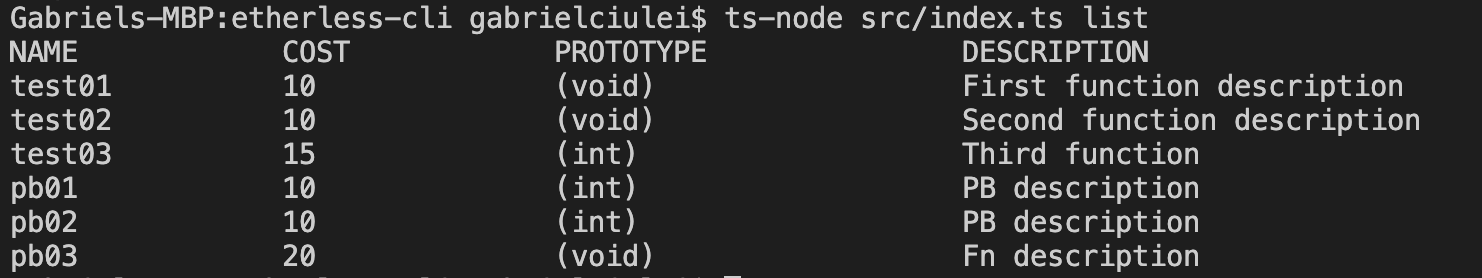
\includegraphics[width=\textwidth]{res/img/Screenshot_list.jpg}
	\caption{List command}
\end{figure}



%\subsubsection{Find}
%The user can search informations about a %specific function already deployed\glo by %another developer, typing the function %name.\\\\
%\centerline{\code{find <function name>}}
%\begin{figure}
%	\centering
%	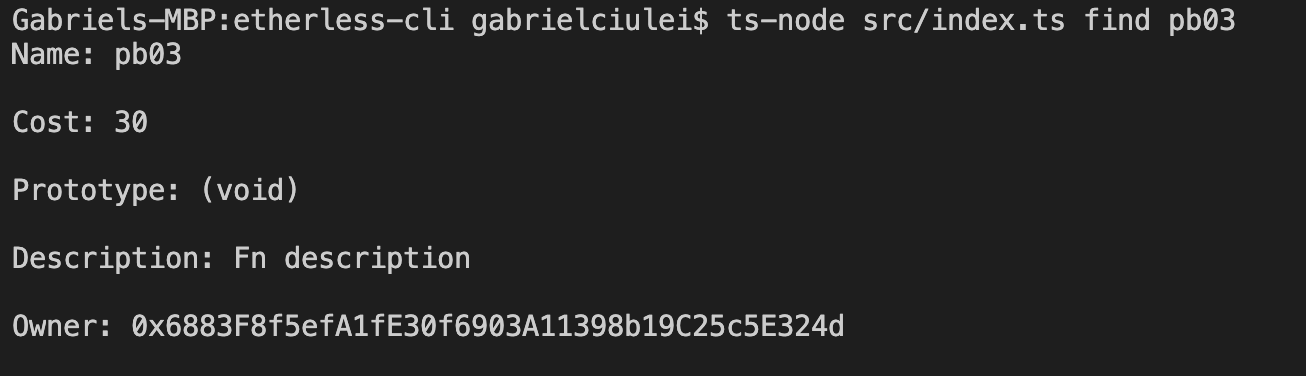
\includegraphics[width=\textwidth]{res/img/Screenshot_find.jpg}
%	\caption{Find command}
%\end{figure}

%\\
%\\aggiungere screen comando

%\subsubsection{Log}
%The user can retrieve all the information about the latest transactions through the command "log".\\\\
%\centerline{\code{log}
%\begin{figure}
%	\centering
%	\includegraphics[width=\textwidth]{res/img/Screenshot_log.jpg}
%	\caption{Log command}
%\end{figure}}
%aggiungere screen comando

\subsubsection{Run}
This command runs myFunction, on \textit{etherless-server}, passing param1, ...paramN as parameters. The parameter order follows the order of the function signature. Run is a synchronous command. Once launched it returns the result of the function or, in case the functions has some execution problems, an exception.\\\\
\centerline{\code{run <functionName> <password> [parameters...]}}
\begin{figure}
	\centering
	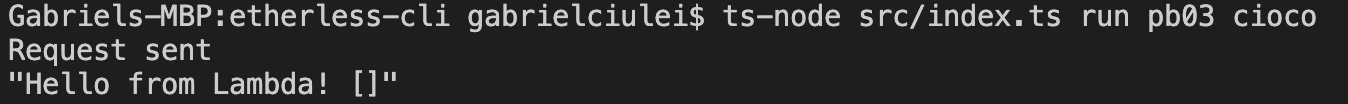
\includegraphics[width=\textwidth]{res/img/Screenshot_run.png}
	\caption{Run command}
\end{figure}
\\
\\

\subsubsection{Deploy\glo}
The command allows the user to deploy\glo to etherless-server the JavaScript function exported in \textit{file.js} under the name "myFunction".\\ 
"myFunction" is also the handler of which the function will be available to the user once deployed. Deploy\glo is a synchronous command. Once launched, it returns only when the deploy\glo is successful or an exception if it encounters some problems.\\
\\
\centerline{\code{deploy <name> <description> <prototype> <cost> <file> <password>}}
\begin{figure}
	\centering
	
\includegraphics[width=\textwidth]{res/img/Screenshot_deploy.png}
	\caption{Deploy command}
\end{figure}





